\documentclass{article}
\usepackage{geometry}
\usepackage{amsmath}
\usepackage{float}
\usepackage{graphicx}
\usepackage{hyperref}
\hypersetup{
    colorlinks=true,
    linkcolor=blue,
    filecolor=magenta,      
    urlcolor=cyan,
}
\usepackage{tikz}
\usetikzlibrary{fit}
\tikzset{
  highlight/.style={rectangle,rounded corners,fill=red!15,draw,
    fill opacity=0.5,thick,inner sep=0pt}
}
\newcommand{\tikzmark}[2]{\tikz[overlay,remember picture,
  baseline=(#1.base)] \node (#1) {#2};}
\newcommand{\Highlight}[1][submatrix]{
    \tikz[overlay,remember picture]{
    \node[highlight,fit=(left.north west) (right.south east)] (#1) {};}
}
\begin{document}
\renewcommand{\vec}[1]{\mathbf{#1}}

\section{Define message passing}

I construct an array of velocities which I pass through the chase routine which computes the position at each iteration.
\[
  velocities = \left(\begin{array}{*1{c}}
    \tikzmark{left}{$v_1$} \tikzmark{right}{} \\
    v_2 \\
    \\
    \\
    v_{N_{vel}}
  \end{array}\right)
  \Highlight[first]
  \qquad
  positions = \left(\begin{array}{*4{c}}
    \tikzmark{left}{$x_{11}$} & x_{12} & \dots & \tikzmark{right}{$x_{1N_{iter}}$} \\
    x_{21} & x_{22} & \dots & x_{2N_{iter}} \\
    \\
    \\
    x_{N_{vel}1} & x_{N_{vel}2} & \dots & x_{N_{vel}N_{iter}}
  \end{array}\right)
\]
\Highlight[second]
\tikz[overlay,remember picture] {
  \draw[->,thick,black,dashed] (first) -- (second) node [pos=0.66,above] {chase};
}
I can manipulate granularity by sending multiple velocities to the chase routine at once.
\[
  velocities = \left(\begin{array}{*1{c}}
    \tikzmark{left}{$v_1$}  \\
    \tikzmark{right}{$v_2$} \\
    \\
    \\
    v_{N_{vel}}
  \end{array}\right)
  \Highlight[first]
  \qquad
  positions = \left(\begin{array}{*4{c}}
    \tikzmark{left}{$x_{11}$} & x_{12} & \dots & x_{1N_{iter}} \\
    x_{21} & x_{22} & \dots & \tikzmark{right}{$x_{2N_{iter}}$} \\
    \\
    \\
    x_{N_{vel}1} & x_{N_{vel}2} & \dots & x_{N_{vel}N_{iter}}
  \end{array}\right)
\]
\Highlight[second]
%
\tikz[overlay,remember picture] {
  \draw[->,thick,black,dashed] (first) -- (second) node [pos=0.66,above] {chase};
}

In static load balancing, processes do jobs where $\mod(i,size)=rank$ where size is the number of processes and rank is the ID of the process.
For static load balancing with granularity, processes do jobs where $\mod(i/N_{vec},size)=rank$ where $N_{vec}$ is the number of grouped jobs.
In dynamic load balancing, the manager assigns workers $N_{vec}$ jobs and waits for a worker to finish.
When a worker is ready, the manager sends the next $N_{vec}$ jobs.
This repeats until all jobs are finished.

\begin{figure}[H]
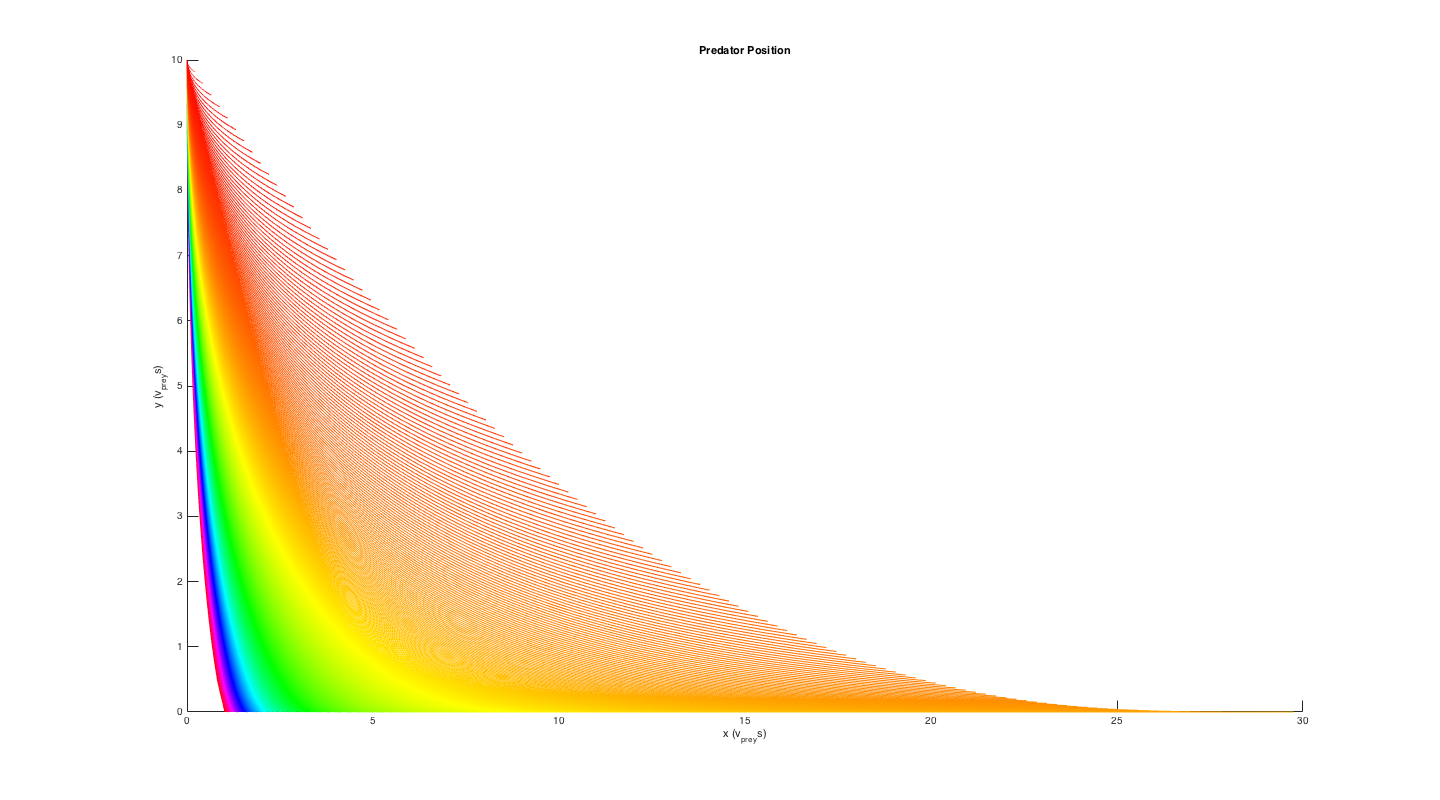
\includegraphics[width=\textwidth]{trajectories.png}
\caption{Trajectories for 1000 velocities from 0 to 10. Red=0, Magenta=10.
View a real time movie \href{run:./trajectories.mp4}{here}.}
\end{figure}

\section{Scalability}

To determine the cost of each job, I define the following:

\begin{align*}
N_{iter} &= \text{Maximum number of time steps} \\
N_{vel} &= \text{Number of predator velocities} \\
v_{min} &= \text{Minimum velocity of predator} \\
v_{max} &= \text{Maximum velocity of predator} \\
t_{max} &= \text{Maximum time given to capture}
\end{align*}

\begin{figure}[H]
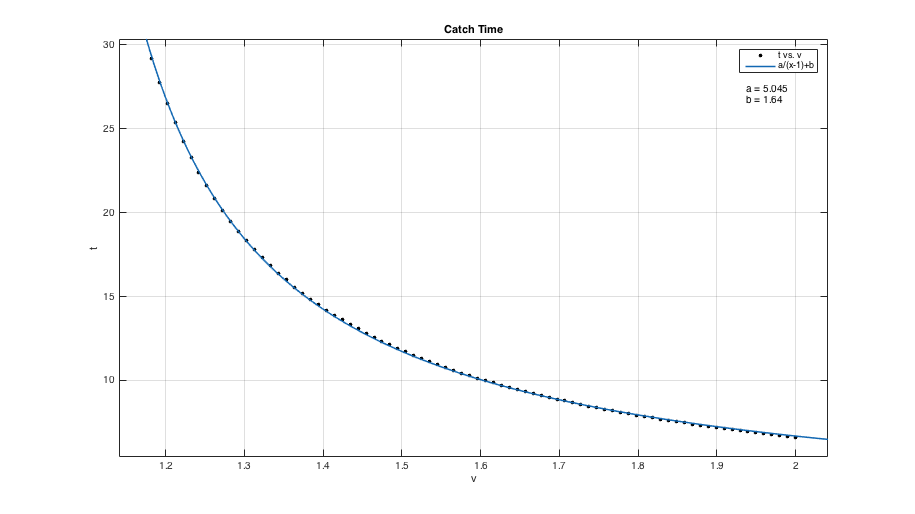
\includegraphics[width=\textwidth]{catch_time.png}
\caption{$N_{iter}=1000$, $N_{vel}=101$, $v_{min}=1$, $v_{max}=2$}
\end{figure}

I used the bisection method to find the minimum velocity of capture.
For $t_{max}=30 s$, I calculated $v_{cap}=1.176585$.
From this, I calculated the total calculation cost.

\begin{align*}
C &= \frac{N_{iter} N_{vel}}{t_{max}}
\left( 
  \int_{v_{min}}^{v_{cap}} t_{max} dv + 
  \int_{v_{cap}}^{v_{max}} (\frac{5.045}{v-1}+1.64)dv
\right) \\
&= N_{iter} N_{vel} \left(
(v_{cap}-v_{min}) + 
\frac{5.045}{t_{max}} \log \left( \frac{v_{max}-1}{v_{cap}-1} \right) + 
\frac{1.64}{t_{max}} (v_{max}-v_{cap})
\right)
\end{align*}

From this, we can see that the calculation cost is proportional to $N_{iter}$ and $N_{vel}$, decreases linearly with $v_{min}$, and increases as $v_{max}+\alpha \log(v_{max}-1)$.

To determine what these values should be, we should consider how much resolution we need for time and for velocity. 
\begin{align*}
\Delta t &= \frac{t_{max}}{N_{iter}} \\
\Delta v &=\frac{v_{max}-v_{min}}{N_{vel}}
\end{align*}

I save all the results in an $N_{iter} \times N_{vel}$ array of complex doubles (16 bytes).
I also have an array of velocities of $N_{vel}$ doubles (8 bytes). The total memory for this is $N_{vel}(8 + 16 N_{iter})$ bytes.
At $N_{vel}=10,000$ and $N_{iter}=10,000$, the memory requirement is already at 1.5GB.
I also made a program that does not save the full trajectory but only the velocities and the time of catch which only requires $16N_{vel}$ bytes of memory.
High resolution is acheived with $N_{vel}=1000$ and $N_{iter}=1000$ and anything more is unnecessary for plots.
The maximum number of processes is $N_{vel}$, in which case 1024 nodes is excessive.

\section{Load Balancing}

As we can see in figure 2, the computation time is much longer for lower velocities. However, in static load balancing, the jobs are divided evenly and each process does approximately the same computation cost.
If we increase granularity though, the jobs are not as well distributed.
This is because a single process will do consecutive velocities.
If consecutive velocities are relatively time consuming, the idle time for other processes may increase.

Jobs that are close to $v=1$ are the most time consuming. Any process that does the most calculations closest to $v=1$ will have to do the most computation. We can use load balancing in this case to distribute the work load. In any case, high granularity is prefered since the cost of using consecutive velocities outweighs the communication latency.

\begin{figure}[H]
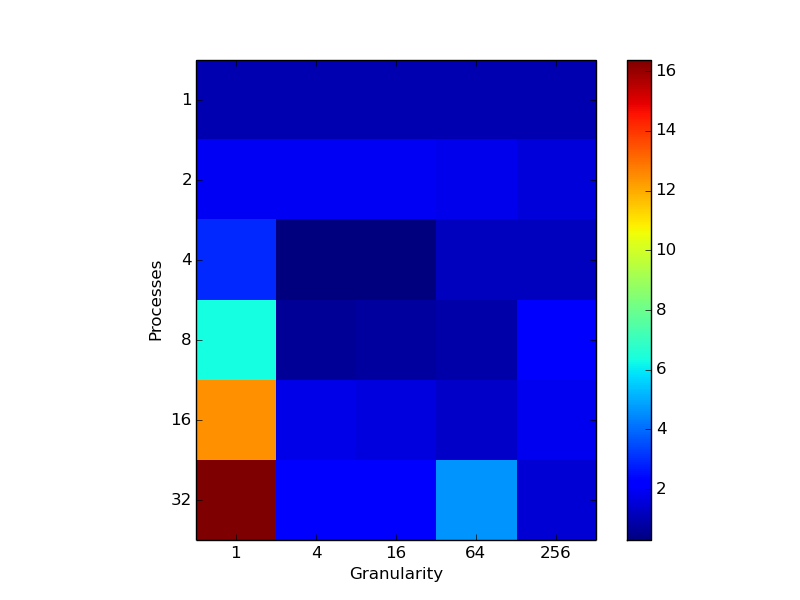
\includegraphics[width=\textwidth]{speedup_static.png}
\caption{Speedup for static load balancing}
\end{figure}

\begin{figure}[H]
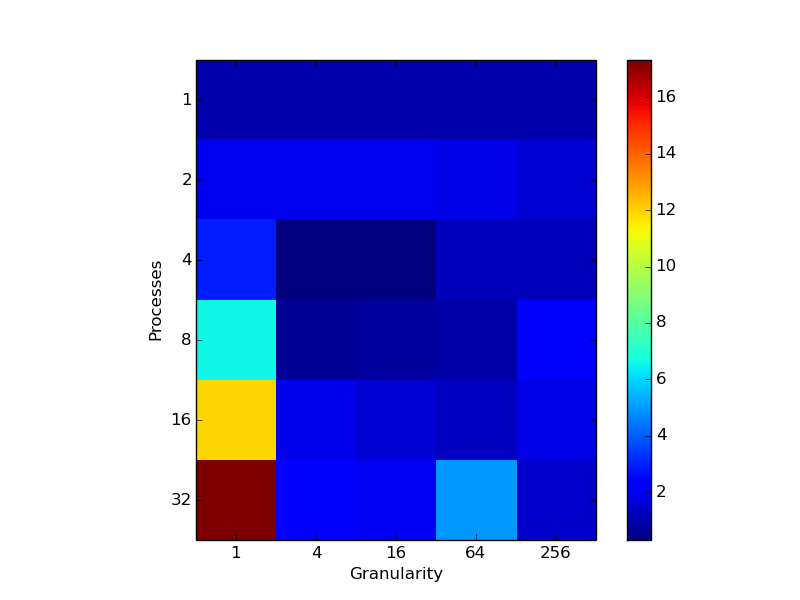
\includegraphics[width=\textwidth]{speedup_dynamic.png}
\caption{Speedup for dynamic load balancing}
\end{figure}

\end{document}